\documentclass[12pt]{article}

\usepackage[a4paper]{geometry} %page size
\usepackage{parskip} %no paragraph indentation
\usepackage{fancyhdr} %fancy stuff in page header
\pagestyle{fancy} 

\usepackage[utf8]{inputenc} %encoding
\usepackage[danish]{babel} %danish letters

\usepackage{graphicx} %import pictures
\graphicspath{ {images/} }
\usepackage{listings} %make lists

\usepackage{amsmath, amssymb, amsfonts, amsthm, mathtools} %doing math
\usepackage{algorithmicx, algpseudocode} %doing pseudocode

\title{
  Title\
  \large Subtitle
}
\author{Asger Andersen}
\date{\today}

\fancyhead{}
\lhead{Miniprojekt 1}
\rhead{Asger Andersen}

%End of preamble
%*******************************************************************************

\begin{document}

\section{Disposition}

Jeg vil gerne gennemgå opgave 1. Jeg vil forsøge at anlægge et perspektiv, hvor jeg fokuserer mere på de overordnede principper og bagvedliggende intutioner end konkrete udregninger.

\begin{itemize}
\item Præsentation og udledning af modellen
\item Definition af ligevægt, og bevis for under hvilke betingelser en affin model har en ligevægt.
\item Udledning af ligevægten for vores model.
\item Definition af stabilitet og redegørelse for betingelserne for, at en affin model har en stabil ligevægt.
\item Udledning af betingelserne for, hvornår ligevægten for vores model er stabil.
\item Fortolkning af resultaterne.
\end{itemize}

(Når jeg bruger egenværdierne, så husk at gennemgå hvad egenværdier er og intuitionen bag det karakteriske polynomien).

 \section{Udregninger}

Vi vil gerne modellere den samlede mængde af forbrug og investinger i år $t$:
\begin{align}
x_t = \begin{pmatrix}
C_t \\ I_t
\end{pmatrix}
\end{align} 

Vi ønsker en simpel model på formen
\begin{align}
x_{t+1} = Mx_t + \gamma, \qquad x_0\in \mathbb{R}^2
\end{align}
altså en model, hvor $x_t$ er en affin funktion af $x_{t-1}$.

Vi forsimpler virkeligheden ved hjælp af tre antagelser:
\begin{align}
Y_t = C_t + I_t \\
C_{t+1} = aY_t + b,\qquad 0<a<1, \quad 0<b \\
I_{t+1} = c(C_{t+1} - C_t), \qquad 0<c
\end{align}
Den første antagelse siger, at nationalproduktet i år $t$ er summen af forbruget og investingerne i år $t$. Den anden antagelse siger, at forbruget i år $t+1$ udgøres af en \textit{fast} andel $a$
af nationalproduktet året før, samt en fast mængde forbrug $b$. Den tredje antagelse siger, at forholdet mellem investeringerne i år $t+1$ og forbrugsstigningen mellem år $t$ og $t+1$ er konstant, nemlig $c$.

Vi omskriver disse ligninger til den ønskede form:
\begin{align}
C_{t+1} = aC_t + aI_t + b \\
I_{t+1} = c(aC_t + aI_t + b - C_t) = (a-1)cC_t + acI_t + bc
\end{align}
hvilket giver
\begin{align}
x_{t+1} = Mx_t + \gamma, \qquad x_0\in \mathbb{R}^2
\end{align}
hvor
\begin{align}
M = \begin{bmatrix}
a && a \\
(a-1)c && ac
\end{bmatrix}, \qquad \gamma = \begin{pmatrix}
b \\ bc
\end{pmatrix}, \qquad 0<b,c,\qquad 0<a<1
\end{align}

Lad os nu bestemme om denne model har en ligevægt og under hvilke betingelser ligevægten er stabil.

Definitionen af ligevægt $x^* \in \mathbb{R}^2$ er
\begin{align}
x^* = Mx^* + \gamma
\end{align}
hvilket er ækvivalent med
\begin{align}
Mx^* - x^* = - \gamma
\end{align}
hvilket er ækvivalent med
\begin{align}
(M - E)x^* = - \gamma
\end{align}
hvilket er ækvivalent med
\begin{align}
x^* = - (M - E)^{-1} \gamma
\end{align}
Altså har modellen en ligevægt, hvis og kun hvis $M-E$ er invertibel, og i så fald er ligevæten givet som ovenfor.

Da 
\begin{align}
\det (M - E) = (a-1)(ac-1) - a(a-1)c = 1-a > 0
\end{align}
så har $(M-E)$ en invers, nemlig
\begin{align}
(M-E)^{-1} = \frac{1}{1-a} \begin{bmatrix}
ac-1 && -a \\
-(a-1)c && a - 1
\end{bmatrix}
\end{align}
og modellen har netop én ligevægt givet ved
\begin{align}
-(M-E)^{-1}\begin{pmatrix}
b\\
bc
\end{pmatrix} =
\begin{pmatrix}
\frac{b}{1-a}\\
0
\end{pmatrix}
\end{align}
For at finde ud af om denne ligevægt er stabil eller ej, vil jeg se nærmere på egenværdierne for $A$. Jeg opskriver derfor det karakteristiske polynomien for $A$:
\begin{align}
\begin{vmatrix}
a - \lambda && a \\
(a-1)c && ac - \lambda
\end{vmatrix} = \\
(a-\lambda)(ac - \lambda) - a(a-1)c =\\ 
\lambda^2 + (-a(c+1))\lambda + ac
\end{align}

Fra hintet i opgavebeskrivelsen ved jeg, at polynomiet har rødder, der er numerisk skarpt mindre end 1, hvis og kun hvis
\begin{align}
|ac| < 1
\end{align}
og
\begin{align}
|-a(c+1)| < 1 + ac
\end{align}
begge gælder.

Da $a,b,c>0$, så er
\begin{align}
|-a(c+1)| < 1 + ac
\end{align}
ækvivalent med
\begin{align}
ac+a < 1 + ac
\end{align}
hvilket er ækvivalent med
\begin{align}
a < 1
\end{align}
hvilket er opfyldt per antagelse. 

Altså har vi, at modellen har en stabil ligevægt, hvis og kun hvis
\begin{align}
c < \frac{1}{a}
\end{align}

Lad os nu fortolke vores resultater. For at vores model skal have en stabil ligevægt og altså konvergere mod denne, når $t\to \infty$, så skal det konstante forhold $c$ mellem vores investeringer og vores forbrugsstigning holde sig under en bestemt grænse, nemlig $\frac{1}{a}$. Hvis $a=0.5$ og vores forbrug altså udgør halvdelen af sidste års nationalprodukt plus $b$, så skal vores investeringer være under dobbelt så store som forbrugsstigningen, hvis modellen skal konvergere. I så fald konvergerer den mod en investeringsmængde på 0 og et årligt forbrug på $b/(1-a)$.


Sætter vi $a=0.48, b=1, c=1.5$, så har modellen en stabil ligevægt, da 
\begin{align}
c = 1.5 < 2.08 = \frac{1}{0.48} = \frac{1}{a}
\end{align}
Altså har vores model i så fald netop én stabil ligevægt, og denne er givet ved
\begin{align}
\begin{pmatrix}
\frac{b}{1-a} \\
0
\end{pmatrix}=
\begin{pmatrix}
\frac{1}{1-0.48} \\
0
\end{pmatrix}= 
\begin{pmatrix}
1.9231 \\
0
\end{pmatrix}
\end{align}
Dette svarer til, hvad vi ser, når vi numerisk fremskriver modellen ud fra disse parametre, og med en startværdi $x_0 = (1.8, 0.4)$:

\begin{center}
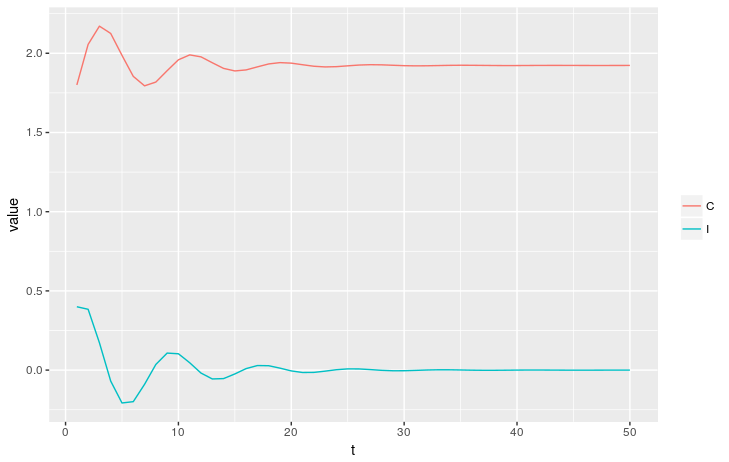
\includegraphics[scale=0.75]{q1p1.png}
\end{center}

Her er værdierne af $C_t$ og $I_t$ for $t=45,...,50$:

\begin{table}[ht]
\centering
\begin{tabular}{rrrr}
  \hline
 & t & C & I \\ 
  \hline
1 &      45 & 1.923166 & -0.000291 \\ 
  2 &      46 & 1.922980 & -0.000279 \\ 
  3 &      47 & 1.922897 & -0.000126 \\ 
  4 &      48 & 1.922930 & 0.000050 \\ 
  5 &      49 & 1.923031 & 0.000151 \\ 
  6 &      50 & 1.923127 & 0.000145 \\ 
   \hline
\end{tabular}
\end{table}

Det ser altså ud til, at $(C_t, I_I)$ konveregerer mod $(1.923, 0)$, når $t$ går mod uendelig.

\end{document}